% !TEX root = ../Report.tex

\subsection{Setup}

The project was created in Python 3, the NiBabel python library was used to convert and import the CT scans and the two architectures were built and trained on Tensorflow and Keras with Tensorflow backend. The tool 3DSlicer was used to display the CT scans and labelmaps and to create the 3D model of the lung and bronchus.

\subsection{Training processes}
The training of both networks was done on a workstation with 64GB of DDR4 RAM and a Nvidia GTX1080Ti GPU. The training process consumed a large amount of computational power and RAM/VRAM storage. The large demand for RAM can be attributed to the fact that the whole training dataset was imported at once instead of loading samples from the disk as required and feeding it to the training process with the above described generator. The training for both networks on the 10 CT scans over 35 epochs took around 10 hours.\newline 
The loss function during training of the DeepMedic architecture is shown in figure \ref{train_deepmedic}. The BCE loss for the lungs converges very fast to an asymptote close to 0. The loss for the bronchus is less stable and decreases slower. It remains higher than the loss for the lungs due to the bronchus being much more complicated and variable across patient scans and is thus more difficult to generalize and segment.\newline
\begin{figure}[h!]
	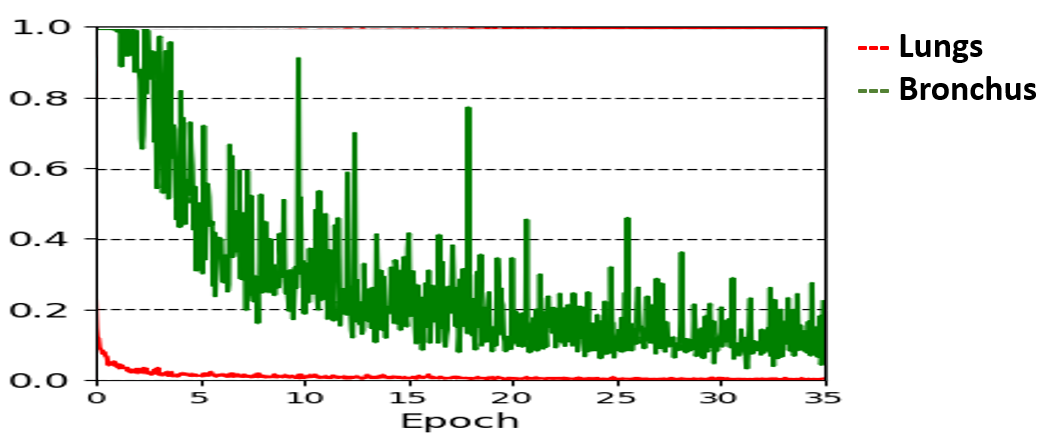
\includegraphics[width=0.49\textwidth, angle=0]{files/deepmedictrain.png}
	\caption{Training process of the DeepMedic architecture. The loss function (BCE) on the training data is shown for the lungs (red) and for the bronchus (green)}
	\label{train_deepmedic}
\end{figure}

The training process for the U-Net architecture is shown in figure \ref{train_unet}. Here the dice loss and the used loss function converge to a asymptote close to 0 on the training set. The metrics on the validation set however do not converge in the same manner. This is caused by overfitting. In some epochs the model creates a too specific representation, overfitting on the training dataset and is therefore not able to get satisfactory results on the validation set. During the training process only models with an improved loss function on the validation set were saved. But in the last 5 epochs the loss function on the validation set decreases to an appropriate value and therefore the model is much more suitable for general predictions on the test set.

\begin{figure}[h!]
	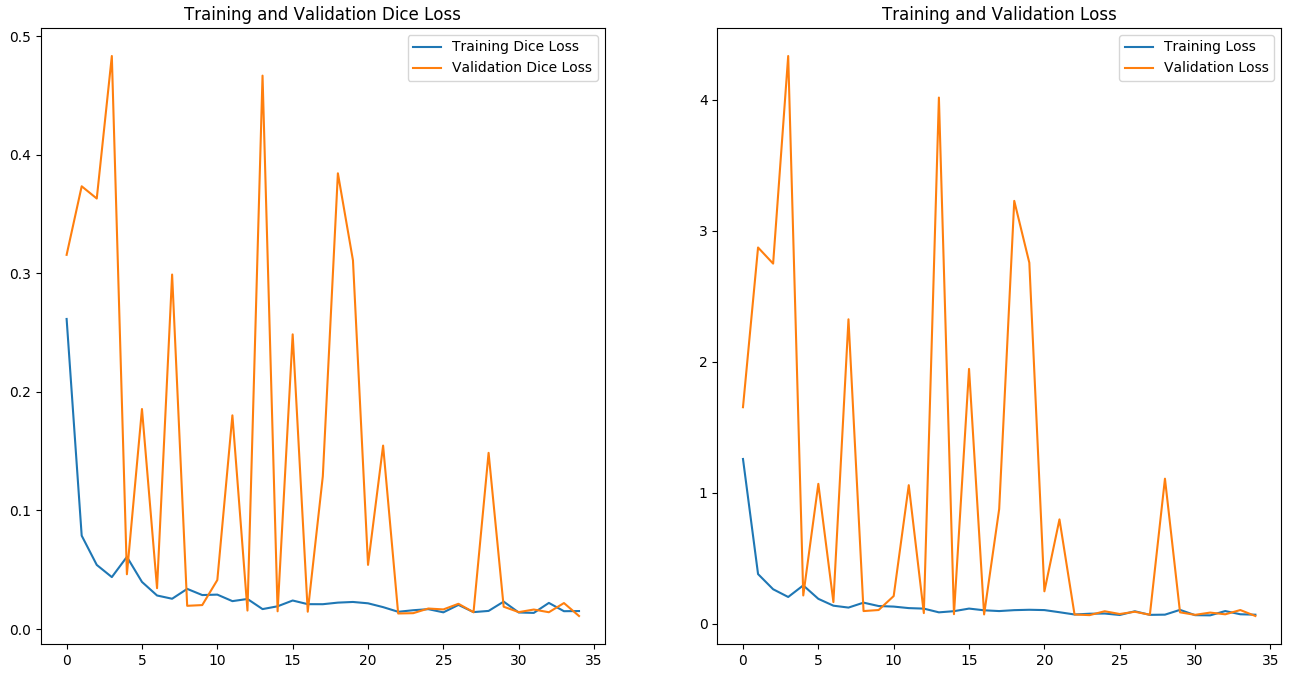
\includegraphics[width=0.49\textwidth, angle=0]{files/jpgunettrain.png}
	\caption{Training process of the U-Net architecture. The dice loss on the training and validation data is shown on the left. The actual loss function ($BCE + dice loss$) is shown on the right.}
	\label{train_unet}
\end{figure}

\subsection{Evaluation of the two architectures}

\begin{figure}[h!]
	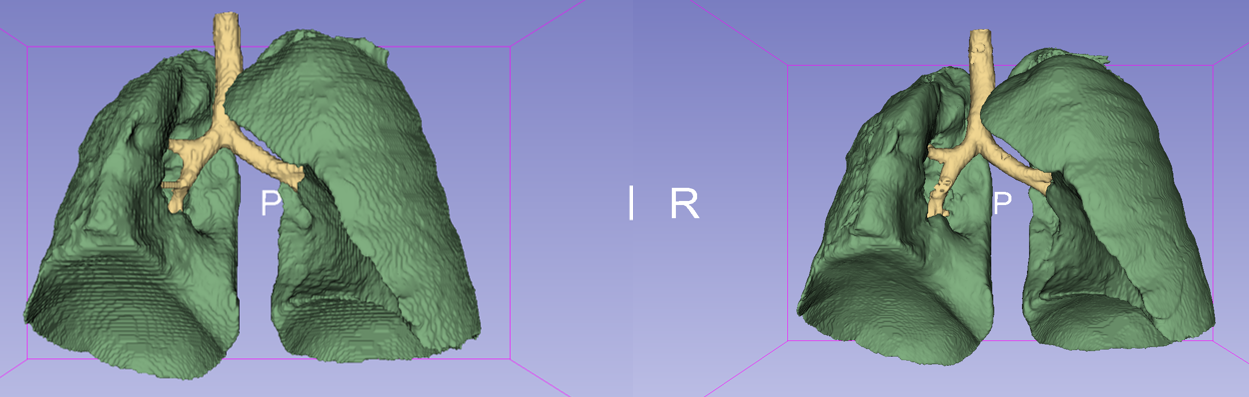
\includegraphics[width=0.49\textwidth, angle=0]{files/preddeepmedic.png}
	\caption{Example prediction of the DeepMedic architecture on one CT scan. The original label map for training is displayed on the left while the prediction of the network is shown on the right.}
	\label{pred_deepmedic}
\end{figure}

For the Deepmedic architecture (shown on figure \ref{pred_deepmedic} above), differences between prediction and actual lung are almost indistinguishable with visual inspection. An interesting point is a very precise representation of the bronchus. DeepMedic is very successful in with the more difficult structure due to its better generalization from the low-resolution CNN path as well as the final statistical step with the CRF, seen in chapter \ref{deepmedic_chapter}. The consistency and accuracy of the DeepMedic bronchus segmentation is the largest practical difference from the U-Net results.\newline

\begin{figure}[h!]
	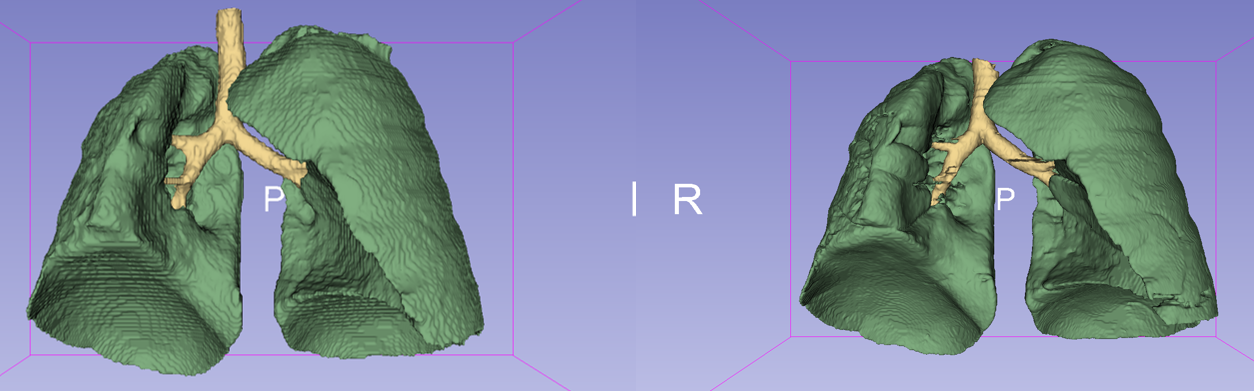
\includegraphics[width=0.49\textwidth, angle=0]{files/predunet.png}
	\caption{Example prediction of the U-Net architecture on one CT scan. The original label map for training is displayed on the left while the prediction of the network is shown on the right.}
	\label{pred_unet}
\end{figure}

Figure \ref{pred_unet} displays an example of the original structure and the predicted scan of the U-Net architecture. The segementation of the bronchus is not as accurate or consistent as it is for Deepmedic. The main reasons for that is that bronchus are more complex, smaller and variable structures. However, the predictions give an appropriate version of the lungs, even slightly better than Deepmedic's ones.\newline\newline

Last part focuses on quantitative analysis over chosen metrics.

comparison of unet and deepmedic

The relatively high Hausdorff can be explained by the metric's high sensitivity to noise in images. As the predicted labelmaps had not been post-processed using methods such as island removal prior to metric calculations any small noise in the predicted labelmap will produce a large Hausdorff distance value.

\begin{table}[h!]
	\caption{Dice Loss, Hausdorff distance and mean distance (on lungs and bronchus) averaged over 20 evaluation CT scans for the DeepMedic and the U-Net architecture.}
	\label{table_result}
	\centering
	\setlength{\tabcolsep}{10pt}
	\renewcommand{\arraystretch}{1.5}
	\begin{tabular}{c c c c}
		\hline 
		Architecture & Dice & Hausdorff & Mean \\
		& Coefficient & distance (mm) & Distance (mm) \\ 
		\hline 
		DeepMedic & 0.968 & 119.50 & 1.45 \\ 
		U-Net & 0.976 & 103.21 & 0.33 \\ 
		\hline
		\newline 
	\end{tabular}

\end{table}
